\chapter{Background}

Consider a simple programming language as defined in figure \ref{fig:bnf_simplelanguage}. In this background chapter we will assign it concrete semantics for actually executing a program written in this language in the concrete. We will then compare this concrete semantics to an abstract interpretation of the language.

\begin{figure}[!htb]
\begin{center}
\begin{tabular}{rcl}
	
program \texttt{p} $\in\mathbb{P}$& ::= & \texttt{A[e] := e}\\
  &$|$&  \texttt{x := e}\\
  &$|$&  \texttt{p$_\mathtt{1}$; p$_\mathtt{2}$}\\
  &$|$&  \texttt{if b then p$_\mathtt{1}$ else p$_\mathtt{2}$}\\
  &$|$&  \texttt{while b then p}\\
  \\
  boolean expression \texttt{b} $\in\mathbb{B}$ & ::= & \texttt{e$_\mathtt{1}$<e$_\mathtt{2}$} $|$  \texttt{e$_\mathtt{1}$<=e$_\mathtt{2}$} $|$ \texttt{!e} $|$ \texttt{e$_\mathtt{1}$==e$_\mathtt{2}$}\\
	\\
	arithmetic expression \texttt{e} $\in\mathbb{E}$ & ::= & \texttt{z} $|$ \texttt{x} $|$ \texttt{A[e]} $|$ \texttt{e$_\mathtt{1}$+e$_\mathtt{2}$} $|$ \texttt{e$_\mathtt{1}$-e$_\mathtt{2}$} $|$ \texttt{e$_\mathtt{1}$*e$_\mathtt{2}$} $|$ \texttt{e$_\mathtt{1}$/e$_\mathtt{2}$}\\

  \\
	numeral \texttt{z}&$\in$&$\mathbb{Z}$\\
	scalar variable name \texttt{x}&$\in$&$\mathbb{X}$\\
	array variable name \texttt{A}&$\in$&$\mathbb{A}$\\
\end{tabular}
\end{center}
\caption{The grammar for a simple example language in Backus--Naur form.}\label{fig:bnf_simplelanguage}
\end{figure}

\section{Program semantics}

Consider the following computer program written in some simple fictive programming language.

\begin{center}
\begin{BVerbatim}
i := 0;
while (i < 10) {
    i := i + 1;
}
\end{BVerbatim}
\end{center}

An experienced programmer might be quick to think they know what this code is supposed to do. They however can only see the syntax of this program and have no knowledge of what the statements actually do in the made-up language. To discover what is happening we first must define the language's semantics. 


\subsection{Environments and Expressions}

Determining the meaning of a particular statement requires us to know the current state of the program. The expression \texttt{i + 1} has an entirely different result, depending on the value of the variable \texttt{i}, which is recorded in the program's concrete scalar variable environment. An environment is defined as a function $\rho\in\mathcal{R}_v$ with $\mathcal{R}_v \triangleq \mathbb{X}\mapsto\mathcal{V}$, where $\mathbb{X}$ is the set of syntactical variable names and $\mathcal{V}$ is the set of values they can take \cite{cousot2011}.

Now consider the simple syntactical expression $\mathtt{e}\in\mathbb{E}$. It only contains scalar constants, scalar variable references and operators. Now $\llbracket\mathtt{e}\rrbracket\rho$ describes the semantics of \texttt{e} in the concrete variable environment $\rho$. The semantics of a variable \texttt{i} is defined as $\llbracket\mathtt{i}\rrbracket\rho=\rho(\mathtt{i})$ and the semantics of a syntactic operator $\circledast$ is defined as $\llbracket\mathtt{e_0\circledast e_1}\rrbracket\rho=\llbracket\mathtt{e_0}\rrbracket\rho \ast\llbracket\mathtt{e_1}\rrbracket\rho$ \cite{scott1971}. 
Imagine a variable environment $\rho$, where $\rho(\mathtt{i})=1$, for example. Our previously mentioned expression \texttt{i + 1} evaluates to:

\begin{equation*}
\begin{aligned}
\llbracket\mathtt{i \;\texttt{+}\; 1}\rrbracket\rho &=\llbracket\mathtt{i}\rrbracket\rho +\llbracket\mathtt{1}\rrbracket\rho \\
& = \rho(\mathtt{i}) + 1\\
& = 1+1\\
& = 2
\end{aligned}
\end{equation*}


\subsection{Transformers}\label{transformers}
A computer program not only contains expressions, but also commands or statements that modify the environment itself. For example, consider the environment $\rho$ where $\rho(\mathtt{i})=1$. After executing the command \texttt{i := i + 1}, the value of the variable \texttt{i} changes and therefore the environment $\rho'$ after the execution of the command is different from $\rho$. We write $\llbracket \texttt{i\;:=\;i\;+\;1} \rrbracket\rho=\rho[\mathtt{i}:=\texttt{i\;+\;1}]=\rho'$, meaning the semantics of the environment $\rho$ after executing an assignment \texttt{i\;:=\;i\;+\;1} is an environment $\rho'$ where all occurrences of \texttt{i} have been replaced by \texttt{i\;+\;1}.

More generally the semantics of an assignment is defined as $\llbracket \texttt{i\;:=\;e} \rrbracket\rho=\rho[\mathtt{i}:=\texttt{e}]$ with $\rho[\mathtt{i}:=\texttt{e}](\mathtt{i})=\llbracket\mathtt{e}\rrbracket\rho$ \cite{cousot2011}. Commands that alter the environment are called transformations. They are basically functions in $\mathcal{R}_v\mapsto\mathcal{R}_v$ \cite{scott1971}.


\section{Abstract Interpretation}

Let us take a look at the equation $8174+2938=x$. We want to determine whether $x$ has a positive or a negative value. Instead of doing mental arithmetic and actually adding $2938$ to $8174$ we almost instinctively know that $x$ must be positive because both its summands are positive. Without realising it, we abstracted the operands of the equation to its sign and calculated it with only this property. When applied to static code analysis, this strategy we just instinctively applied, is called abstract interpretation. Its main idea is that for proving a program's properties it is not necessary to run it with concrete values. Instead it can be run on the examined properties \cite{cousot2023, cousot1977}.


\subsection{Properties}

Consider a set of entities $\mathcal{E}$. A formal property $P\subseteq \wp(\mathcal{E}) $ is a set of entities that have this property \cite[chapter 8]{cousot2021}. With the set of integers as our set of entities $\mathcal{E}=\mathbb{Z}$, our ``positive'' property is defined as $P_{pos}=\{z\in \mathcal{E} \;|\; 0<z\}$ and we can define some more semantic properties like in table \ref{table:properties}.
\begin{table}[hbt]
\begin{center}
  \begin{tabular}{l|l}
  $\mathsf{false}$ & $\emptyset$\\
   $P_{0}$ & $\{0\}$\\
   $P_{pos}$ & $\{z\in \mathbb{Z} \;|\; 0<z\}$\\
   $P_{neg}$ & $\{z\in \mathbb{Z} \;|\; 0>z\}$\\
   $P_{pos0}$ & $\{z\in \mathbb{Z} \;|\; 0\leq z\}$\\
   $P_{neg0}$ & $\{z\in \mathbb{Z} \;|\; 0\geq z\}$\\
   $P_{even}$ & $\{z\in \mathbb{Z} \;|\; \exists k\in\mathbb{Z}:2k=z \}$ \\
   $P_{odd}$ & $\{z\in \mathbb{Z} \;|\; \exists k\in\mathbb{Z}:2k+1=z \}$ \\
   $P_{pos\_even}$ & $\{z\in \mathbb{Z} \;|\; z>0 \wedge \exists k\in\mathbb{Z}:2k=z \} = P_{pos} \cap P_{even}$ \\
   $\vdots$ &$\vdots$\\
   $\mathsf{true}$ & $\mathbb{Z}$\\
  \end{tabular}
  \caption{An incomplete selection of properties for $\mathbb{Z}$.}\label{table:properties}
  \end{center}
\end{table}

We call a property $P$ ``stronger'' than $P'$ (or $P'$ ``weaker'' than $P$) if $P\subseteq P'$. Its set representation contains less elements and we therefore have more information about an element that fulfils said property. The weakest property is the $\mathsf{true}$ property that is satisfied by alle elements and the strongest is $\mathsf{false}$ which is satisfied by none \cite[chapter 8]{cousot2021}. Not all properties from $\wp(\mathcal{E})$ carry a semantic meaning. We therefore only consider the set of properties of interest $C\subseteq\wp(\mathcal{E})$. If we want to analyse the signs of integers this could be $C_{sign}=\{\mathsf{false}, P_{0}, P_{pos}, P_{neg}, P_{pos0}, P_{neg0}, P_{not0}, \mathsf{true}\}$. The poset  $\langle C,\subseteq\rangle$ is called the ``concrete domain''.

\subsection{Abstraction}\label{sec:abstractinterpretation:abstraction}

Now consider a set of abstract properties $A$. This is not a power set of concrete values anymore but a set of purely semantic symbols that represent abstract properties. If there exists a Galois connection $\langle C,\subseteq\rangle \galois{\alpha}{\gamma}\langle A\sqsubseteq\rangle$, we call $\langle A\sqsubseteq\rangle$ the abstract domain, $\alpha\in C\to A$ the abstraction function and $\gamma\in A\to C$ the concretisation function \cite[chapter 11]{cousot2021}. To put the working principle of Galois connections into simple terms: $A$'s elements abstract $C$'s elements and $\sqsubseteq$ works analogous in the abstract to $\subseteq$ in the concrete. More formally: $\forall P_C\in C:\forall P_A \in A:\alpha(P_C)\sqsubseteq P_A \Longleftrightarrow P_C \subseteq \gamma(P_A)$.

\begin{figure}[htb]
	\begin{center}
		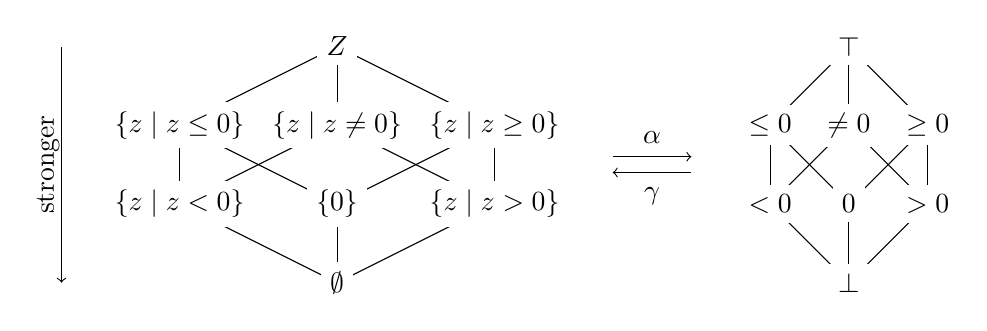
\begin{tikzpicture}
			% Concrete domain
			\draw (-4.5,0) -- (-6.5,1);
            \draw (-4.5,0) -- (-4.5,1);
            \draw (-4.5,0) -- (-2.5,1);
            \draw (-4.5,3) -- (-6.5,2);
            \draw (-4.5,3) -- (-4.5,2);
            \draw (-4.5,3) -- (-2.5,2);
            
            \draw (-4.5,1) -- (-6.5,2);
            \draw (-4.5,1) -- (-2.5,2);
            \draw (-6.5,1) -- (-6.5,2);
            \draw (-2.5,1) -- (-2.5,2);
            \draw (-4.5,2) -- (-6.5,1);
            \draw (-4.5,2) -- (-2.5,1);
            
            \draw (-4.5,0) node[fill=white!5] {$\emptyset$};
            \draw (-6.5,1) node[fill=white!5] {$\{z\;|\;z<0\}$};
            \draw (-4.5,1) node[fill=white!5] {$\{0\}$};
            \draw (-2.5,1) node[fill=white!5] {$\{z\;|\;z>0\}$};
            \draw (-6.5,2) node[fill=white!5] {$\{z\;|\;z\leq0\}$};
            \draw (-4.5,2) node[fill=white!5] {$\{z\;|\;z\neq0\}$};
            \draw (-2.5,2) node[fill=white!5] {$\{z\;|\;z\geq0\}$};
            \draw (-4.5,3) node[fill=white!5] {$\mathbb{Z}$};

			% Abstract domain
            \draw (2,0) -- (1,1);
            \draw (2,0) -- (2,1);
            \draw (2,0) -- (3,1);
            \draw (2,3) -- (1,2);
            \draw (2,3) -- (2,2);
            \draw (2,3) -- (3,2);
            
            \draw (2,1) -- (1,2);
            \draw (2,1) -- (3,2);
            \draw (1,1) -- (1,2);
            \draw (3,1) -- (3,2);
            \draw (2,2) -- (1,1);
            \draw (2,2) -- (3,1);
            
            \draw (2,0) node[fill=white!5] {$\perp$};
            \draw (1,1) node[fill=white!5] {$<0$};
            \draw (2,1) node[fill=white!5] {$0$};
            \draw (3,1) node[fill=white!5] {$>0$};
            \draw (1,2) node[fill=white!5] {$\leq0$};
            \draw (2,2) node[fill=white!5] {$\neq0$};
            \draw (3,2) node[fill=white!5] {$\geq0$};
            \draw (2,3) node[fill=white!5] {$\top$};
            
            
            % Arrows
            \draw (-0.5,1.85) node {$\alpha$};
            \draw [->](-1,1.6) -- (0,1.6);
            \draw [<-](-1,1.4) -- (0,1.4);
            \draw (-0.5,1.1) node {$\gamma$};
            
            \draw [<-](-8,0) -- (-8,3);
            \draw (-8.17,1.5) node[rotate=90] {stronger};
        \end{tikzpicture}
        \caption{The sign properties of the concrete integer domain (left) next to the abstract sign domain (right) as a Hasse diagram. }
	\end{center}
\end{figure}

\subsection{Property Transformers}

When executing a computer program in the concrete, there are transformer semantics in


\begin{figure}[htb]
	\begin{center}
		\begin{tikzpicture}
%            

         \node [circle] (A)  at (0,0)    {c};
  		 \node [circle] (B)  at (4,0)    {c'};
  		 \node [circle] (C)  at (0,2)    {a};
  		 \node [circle] (D)  at (4,2)    {a};
  		 
  		 \draw [->] (A) -- (B); 
  		 \draw [->] (C) -- (D); 
  		 \draw [->] (A) to [bend left=30] node[left]{$\alpha$}  (C); 
  		 \draw [->] (C) to [bend left=30] node[right]{$\gamma$} (A); 
  		 \draw [->] (B) to [bend left=30] node[left]{$\alpha$} (D); 
  		 \draw [->] (D) to [bend left=30] node[right]{$\gamma$} (B); 
  		 
  		 
  		 \draw [->] (A) -- (B); 
  		 \draw [->] (A) -- (B); 
  		 \draw [->] (A) -- (B); 
         
        \end{tikzpicture}
        \caption{Lorem Ipsum}.
	\end{center}
\end{figure}



\begin{table}[hbt]
\begin{center}
\begin{tabular}{c|c|c|c|c|c|c|c|c}
            $\times_\pm$& $\perp$ & $<0$    & $0$     & $>0$    & $\leq0$ & $\neq0$ & $\geq0$ & $\top$  \\ \hline
            $\perp$ & $\perp$ & $\perp$ & $\perp$ & $\perp$ & $\perp$ & $\perp$ & $\perp$ & $\perp$ \\
            $<0$    & $\perp$ & $>0$    & $0$     & $<0$    & $\geq0$ & $\neq0$ & $\leq0$ & $\top$  \\
            $0$     & $\perp$ & $0$     & $0$     & $0$     & $0$     & $0$     & $0$     & $0$     \\
            $>0$    & $\perp$ & $<0$    & $0$     & $>0$    & $\leq0$ & $\neq0$ & $\geq0$ & $\top$  \\
            $\leq0$ & $\perp$ & $\geq0$ & $0$     & $\leq0$ & $\geq0$ & $\top$  & $\leq0$ & $\top$  \\
            $\neq0$ & $\perp$ & $\neq0$ & $0$     & $\neq0$ & $\top$  & $\neq0$ & $\top$  & $\top$  \\
            $\geq0$ & $\perp$ & $\leq0$ & $0$     & $\geq0$ & $\leq0$ & $\top$  & $\geq0$ & $\top$  \\
            $\top$  & $\perp$ & $\top$  & $0$     & $\top$  & $\top$  & $\top$  & $\top$  & $\top$ 
        \end{tabular}
  \caption{A table showcasing the result of the abstract property transformer $\times_\pm$ which is an abstraction of the concrete multiplication operator.}\label{table:multiply}
  \end{center}
\end{table}

\subsection{Fixpoint analysis}

\subsection{The Interval Domain}
asdf

\begin{figure}[htb]
	\begin{center}
		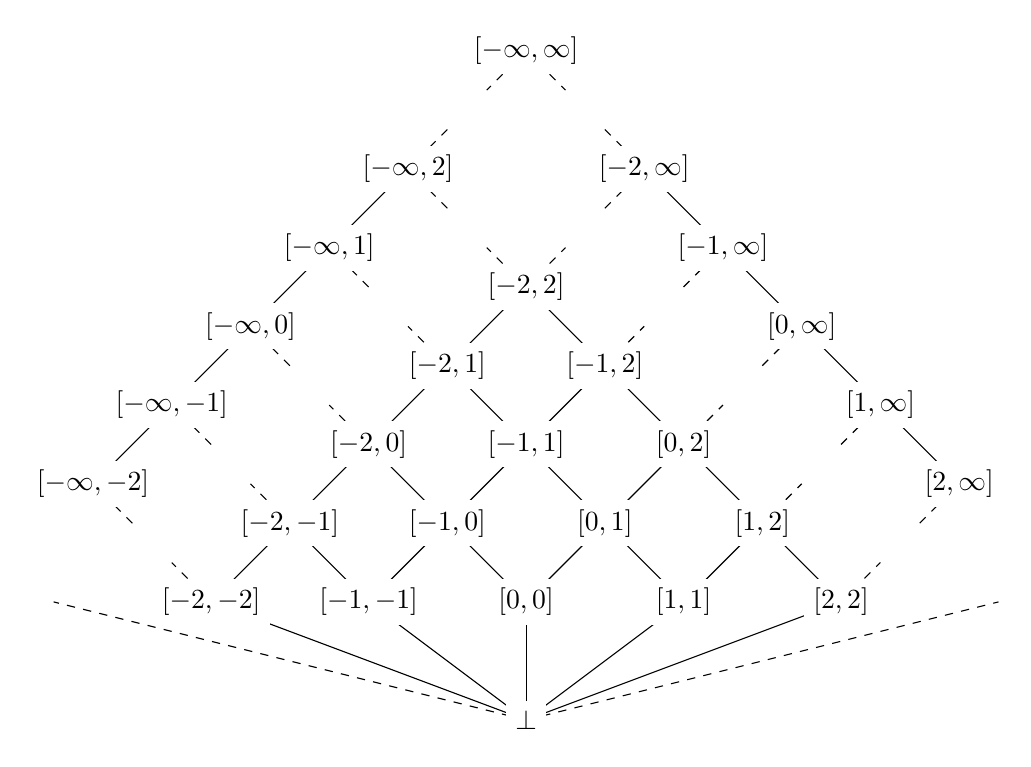
\begin{tikzpicture}
            \draw (0,0) -- (0,1.5);
            \draw (0,0) -- (2,1.5);
            \draw (0,0) -- (4,1.5);
            \draw (0,0) -- (-2,1.5);
            \draw (0,0) -- (-4,1.5);
            \draw (0,0)[dashed] -- (-6,1.5);
            \draw (0,0)[dashed] -- (6,1.5);
            
            \draw (2,1.5) -- (1,2.5);
            \draw (2,1.5) -- (3,2.5);
            \draw (4,1.5) -- (3,2.5);
            \draw (0,1.5) -- (1,2.5);
            \draw (0,1.5) -- (-1,2.5);
            \draw (-2,1.5) -- (-1,2.5);
            \draw (-2,1.5) -- (-3,2.5);
            \draw (-4,1.5) -- (-3,2.5);
            
            \draw (1,2.5) -- (0,3.5);
            \draw (1,2.5) -- (2,3.5);
            \draw (3,2.5) -- (2,3.5);
            \draw (-1,2.5) -- (0,3.5);
            \draw (-1,2.5) -- (-2,3.5);
            \draw (-3,2.5) -- (-2,3.5);
            
            \draw (2,3.5) -- (1,4.5);
            \draw (0,3.5) -- (1,4.5);
            \draw (0,3.5) -- (-1,4.5);
            \draw (-2,3.5) -- (-1,4.5);
            
            \draw (-1,4.5) -- (0,5.5);
            \draw (1,4.5) -- (0,5.5);
            
            \draw (-4,1.5)[dashed] -- (-4.5,2);
            \draw (-5,2.5)[dashed] -- (-5.5,3);
            
            \draw (-3,2.5)[dashed] -- (-3.5,3);
            \draw (-4,3.5)[dashed] -- (-4.5,4);
            
            \draw (-2,3.5)[dashed] -- (-2.5,4);
            \draw (-3,4.5)[dashed] -- (-3.5,5);
            
            \draw (-1,4.5)[dashed] -- (-1.5,5);
            \draw (-2,5.5)[dashed] -- (-2.5,6);
            
            \draw (0,5.5)[dashed] -- (-0.5,6);
            \draw (-1,6.5)[dashed] -- (-1.5,7);
           
            \draw (4,1.5)[dashed] -- (4.5,2);
            \draw (5,2.5)[dashed] -- (5.5,3);
            
            \draw (3,2.5)[dashed] -- (3.5,3);
            \draw (4,3.5)[dashed] -- (4.5,4);
            
            \draw (2,3.5)[dashed] -- (2.5,4);
            \draw (3,4.5)[dashed] -- (3.5,5);
            
            \draw (1,4.5)[dashed] -- (1.5,5);
            \draw (2,5.5)[dashed] -- (2.5,6);
            
            \draw (0,5.5)[dashed] -- (0.5,6);
            \draw (1,6.5)[dashed] -- (1.5,7);
            
            \draw (-5.5,3) -- (-1.5,7);
            \draw (5.5,3) -- (1.5,7);
            
            \draw (-1,7.5)[dashed] -- (-1.5,7);
            \draw (1,7.5)[dashed] -- (1.5,7);
            
            \draw (0,8.5)[dashed] -- (-0.5,8);
            \draw (0,8.5)[dashed] -- (0.5,8);
            
            \draw (0,0) node[fill=white!5] {$\perp$};
            \draw (0,1.5) node[fill=white!5] {$[0,0]$};
            \draw (2,1.5) node[fill=white!5] {$[1,1]$};
            \draw (4,1.5) node[fill=white!5] {$[2,2]$};
            \draw (-2,1.5) node[fill=white!5] {$[-1,-1]$};
            \draw (-4,1.5) node[fill=white!5] {$[-2,-2]$};
            
            \draw (1,2.5) node[fill=white!5] {$[0,1]$};
            \draw (3,2.5) node[fill=white!5] {$[1,2]$};
            \draw (-1,2.5) node[fill=white!5] {$[-1,0]$};
            \draw (-3,2.5) node[fill=white!5] {$[-2,-1]$};
            
            \draw (2,3.5) node[fill=white!5] {$[0,2]$};
            \draw (0,3.5) node[fill=white!5] {$[-1,1]$};
            \draw (-2,3.5) node[fill=white!5] {$[-2,0]$};
            
            \draw (1,4.5) node[fill=white!5] {$[-1,2]$};
            \draw (-1,4.5) node[fill=white!5] {$[-2,1]$};
            
            \draw (0,5.5) node[fill=white!5] {$[-2,2]$};
            
            
            \draw (-5.5,3) node[fill=white!5] {$[-\infty,-2]$};
            \draw (-4.5,4) node[fill=white!5] {$[-\infty,-1]$};
            \draw (-3.5,5) node[fill=white!5] {$[-\infty,0]$};
            \draw (-2.5,6) node[fill=white!5] {$[-\infty,1]$};
            \draw (-1.5,7) node[fill=white!5] {$[-\infty,2]$};
            
            
            \draw (5.5,3) node[fill=white!5] {$[2,\infty]$};
            \draw (4.5,4) node[fill=white!5] {$[1,\infty]$};
            \draw (3.5,5) node[fill=white!5] {$[0,\infty]$};
            \draw (2.5,6) node[fill=white!5] {$[-1,\infty]$};
            \draw (1.5,7) node[fill=white!5] {$[-2,\infty]$};
            
            \draw (0,8.5) node[fill=white!5] {$[-\infty,\infty]$};
         
        \end{tikzpicture}
        \caption{The interval abstract domain as a Hasse diagram \cite{cousot1977}}.\label{fig:intervaldomain}
	\end{center}
\end{figure}

\section{FunArray}
\subsection{Functors}
\subsection{Abstractions}
\subsection{Segmentation Functor: The FunArray}
